\documentclass[instructions]{./Packages/uqthesis}
% ***************************************************
% LaTeX Packages
% ***************************************************
% This file defines the document design.
% Usually it is not necessary to edit this file, but you can use it to change aspects of the design if you want.

%There are essential packages that are contained within the uqthesis.cls which are integral to the template - These must not be deleted.  A list of these packages can be found in the README.tet file

%The packages below are optional, please add or alter as required.

\usepackage{cite}				 %Allows abbreviated numerical citations.
\usepackage{pdfpages}			 %Allows you to include full-page pdfs.
\usepackage{wrapfig}			 %Lets you wrap text around figures.
\usepackage{bm} 				 %Bolded maths characters.
\usepackage{upgreek}			 %Upright Greek characters.
\usepackage{dsfont}				 %Double-struck fonts.
\usepackage{simplewick}			 %For typesetting Wick contractions.
\usepackage{mathtools}		     %Can be used to fine-tune the maths presentation.	
\usepackage{framed}			     %For boxed text.
\usepackage{microtype}			 %pdfLaTeX will fix your kerning.
\usepackage{marvosym}			 %Include symbols (like the Euro symbol, etc.).
\usepackage{color}				 %Nice for scalable pdf graphics using InkScape.
\usepackage{transparent}	     %Nice for scalable pdf graphics using InkScape.
\usepackage{placeins}			 %Lets you put in a \FloatBarrier to stop figures floating past this command.
\usepackage{mdframed,mdwlist}    %Use these for nice lists (less white space).
\usepackage{graphicx}            %Enhanced support for graphics.
\usepackage{float}               %Improved interface for floating objects. 
\usepackage{longtable}           %Allow tables to flow over page boundaries.
\usepackage{mathdots}            %Changed the basic LaTeX and plain TeX commands.
\usepackage{eucal}               %Font shape definitions to use the Euler script symbols in math mode.
\usepackage{array}               %Extending the array and tabular environments.
\usepackage{stmaryrd}            %The StMary’s Road symbol font.
\usepackage{amsthm}              %St Mary Road symbols for theoretical computer science. 
\usepackage{pifont}              %Access to PostScript standard Symbol and Dingbats fonts.
\usepackage{lipsum}              %Easy access to the Lorem Ipsum dummy text.
\usepackage{enumerate}           %Enumerate with redefinable labels. 
\usepackage[all]{xy}             %This is a special package for drawing diagrams.
\usepackage{amsmath}             %ATypesetting theorems (AMS style).
\usepackage{amssymb}             %Provided an extended symbol collection.
\usepackage[utf8]{inputenc}      %Allowed all displayable utf8 characters to be available as input.
\usepackage{fancyhdr}            %Extensive control of page headers and footers.
\usepackage{blindtext}           %Produced 'blind' text for testing.
\usepackage{tikz}                %To create graphic elements.
\usepackage[figuresright]{rotating}	%Allows large tables to be rotated to landscape.
\usetikzlibrary{shapes.geometric, arrows}
%You can add more packages here if you need


%This defines some macros that implement Latin abbreviations
%COMMENT OUT OR DELETE IF UNDESIRED.
\newcommand{\via}{\textit{via}} %Italicised via.
\newcommand{\ie}{\textit{i.e.}} %Literally.
\newcommand{\eg}{\textit{e.g.}} %For example.
\newcommand{\etc}{\textit{etc.}} %So on...
\newcommand{\vv}{\textit{vice versa}} %And the other way around.
\newcommand{\viz}{\textit{viz}.} %Resulting in.
\newcommand{\cf}{\textit{cf}.} %See, or 'consistent with'.
\newcommand{\apr}{\textit{a priori}} %Before the fact.
\newcommand{\apo}{\textit{a posteriori}} %After the fact.
\newcommand{\vivo}{\textit{in vivo}} %In the flesh.
\newcommand{\situ}{\textit{in situ}} %On location.
\newcommand{\silico}{\textit{in silico}} %Simulation.
\newcommand{\vitro}{\textit{in vitro}} %In glass.
\newcommand{\vs}{\textit{versus}} %James \vs{} Pete.
\newcommand{\ala}{\textit{\`{a} la}} %In the manner of...
\newcommand{\apriori}{\textit{a priori}} %Before hand.
\newcommand{\etal}{\textit{et al.}} %And others, with correct punctuation.
\newcommand{\naive}{na\"\i{}ve} %Queen Amidala is young and \naive{}.

\footskip 30pt
\title{Prolog Optimizations in GraalVM}
\author{Thi Thuy Tien Nguyen}
\currentdegrees{Master of Computer Science (Management)}
\orcid{\href{add your ORCID url here}{Candidate's ORCID}}
\date{12 September 2024}
\school{School of Electrical Engineering and Computer Science}
\university{The University of Queensland}

\titleformat{\chapter}{\LARGE\bfseries}{\thechapter}{1em}{\LARGE}
\titlespacing{\chapter}{0pt}{-10pt}{5pt}
\titlespacing{\section}{0pt}{8pt}{5pt}
\titlespacing{\subsection}{0pt}{10pt}{5pt}
\renewcommand{\contentsname}{\vspace{-50pt} \hfill\bfseries\LARGE TABLE OF CONTENTS \hfill \vspace{-10pt}}
\renewcommand{\sectionmark}[1]{\markboth{\thesection~#1}{}}
\begin{document}
\frontmatter
\maketitle
\thispagestyle{empty}

\clearpage

\begin{KeepFromToc}
    \setcounter{page}{0} %reset the page counter
    \tableofcontents
\end{KeepFromToc}
\clearpage
\openany

\mainmatter

\chapter[Abstract]{Abstract}

\noindent
Compiler optimizations are critical for enhancing program execution speed and overall performance. This thesis proposes integrating Prolog-based optimization techniques into the GraalVM compiler framework to potentially enhance compiler performance. The approach involves developing a Prolog-based optimizer that translates GraalVM’s intermediate representation (IR) of programs into Prolog facts and defines optimization rules using Prolog’s declarative syntax. By querying these rules within the GraalVM compiler, the proposal aims to explore how Prolog’s logic programming capabilities can improve the expressiveness and effectiveness of compiler optimizations. The study seeks to assess the feasibility of this integration, examining how Prolog’s declarative nature might contribute to more sophisticated and potentially more efficient optimization strategies compared to traditional imperative methods. This approach could lead to advancements in compiler technology and open new avenues for research in the optimization phase of compilation. The project spans 30 weeks, divided into two semesters and four phases: Project Proposal, Proof of Concept, Extension and Evaluation, and Report and Demonstration, with 10 hours of work per week. The first semester focused on initial research and development of a proof of concept, and the second half on refining, expanding and preparing the final deliverables.
\chapter[Introduction]{Introduction}

Compiler optimizations seek to improve program execution speed and overall performance, which can result in substantial cost savings for large-scale organizations, potentially reducing infrastructure expenses by millions annually. This project aims to assess the feasibility of implementing an optimizer in logic programming language within the GraalVM compiler framework. Specifically, this project examines the integration of GraalVM Ahead-of-Time (AOT) compiler optimizations with Prolog. The project works with AOT due to its advantages over Just-In-Time (JIT) compilation, which involves runtime code compilation that incurs higher overhead in terms of CPU and memory usage and introduces delays through dynamic optimization and profiling. In contrast, AOT compilation completes all compilation and optimizations at build time with minimal runtime overhead. 

Logic programming languages with declarative specifications allow programs to be analyzed efficiently through queries, enabling the implementation of code optimization that would otherwise be difficult to achieve. By focusing on what needs to be achieved rather than how to achieve it, declarative approaches offer greater clarity and intuitiveness. This inherent simplicity and readability facilitate the experimentation and development of new optimization rules, as well as the maintenance of existing ones. Additionally, declarative code is easier to debug, test, and ensure correctness because it is more straightforward and easier to follow. Previous research has extensively utilized Datalog, a prominent logic programming language, for different levels of program analysis \cite{Bravenboer2009,Tonder2021,Lam2005,Benton2007}. However, there is a notable lack of prior work regarding the application of logic programming languages for the optimization and transformation of code. Spinellis’ work in 1999 explored an alternative method for expressing optimizations through declarative specifications, as opposed to traditional imperative code \cite{Spinellis1999}. However, Spinellis’s work was limited to a rudimentary prototype of an optimizer with a ``single optimization specification" and ``limited flow-of-control optimizations" \cite{Spinellis1999}.

The proposed approach involves three main steps. First, optimization rules are defined as Prolog facts and predicates, focusing on canonicalization to standardize the IR code and conditional elimination to remove redundant expressions. Second, the Prolog fact generator parses the IR and converts it into Prolog facts, ensuring compatibility with optimization rules for effective query-based optimization. Finally, the Prolog-based optimizer is developed in Java to recursively query these rules, apply transformations, and refine the IR iteratively. As each optimization is applied, the IR is updated and reconstructed based on the optimized Prolog facts, leading to an improved representation of the program. To ensure correctness, a comprehensive test suite will be created to verify Prolog rule functionality, validate generated facts, and ensure the correctness of the optimized code. The performance will be evaluated based on execution speed, resource usage, and optimization throughput, alongside an assessment of whether Prolog’s declarative syntax improves optimization expressibility, documentation, comprehension, and maintenance.

\chapter[Background and Related Works]{Background}

\section{Background Materials}
\subsection{Ahead-of-time (AOT) Compilation}
In the Java Virtual Machine (JVM), byte code compilation can occur either at build time or runtime. Ahead-of-Time (AOT) compilation involves translating the byte code into machine code before execution, resulting in a fully compiled binary that is immediately executable \cite{Wade2017}. In contrast, Just-In-Time (JIT) Compilation defers the translation until runtime if at all, dynamically converting Java bytecodes into machine code within the Java Virtual Machine (JVM) and optimizing frequently executed code paths to enhance performance \cite{Wade2017}. AOT compilation generally requires longer build times but offers rapid startup and predictable performance, making it suitable for applications where quick initialization is critical. JIT compilation, while benefiting from shorter build times, incurs longer startup periods but allows for more complex optimizations based on runtime profiling data.

JIT compilation enables techniques such as speculative optimizations, which make assumptions about a program’s behavior to apply performance-enhancing transformations based on runtime profiling. Although these optimizations can significantly improve performance by optimizing frequently executed code paths, incorrect assumptions may necessitate deoptimizations, which revert the code to a less optimized but more reliable version \cite{Duboscq2013Inproceedings}. This can complicate the program's IR by adding additional nodes and edges to accommodate these transformations \cite{Duboscq2013Inproceedings}. In this project, the emphasis will be on AOT compilation, where speculative optimizations are excluded \cite{Wimmer2019}, resulting in a simpler IR without the need for deoptimization.

\subsection{GraalVM Compiler Optimizations}

In GraalVM, the compilation process is divided into two main phases. The first phase, involving the Graal IR, handles most of the high-level optimizations. This phase is further organized into three tiers: high-tier for high-level optimizations, mid-tier for memory-focused enhancements, and low-tier for low-level IR (LIR) conversion \cite{Graal2021}. This project will primarily concentrate on high-tier optimizations within the GraalVM, beginning with the canonicalization phase.

Canonicalization, an essential early phase in the optimization process, focuses on transforming code into a standardized format and eliminating redundancies. This transformation simplifies and facilitates the application of subsequent optimizations. Examples of canonicalization include:

\begin{description}
    \item \textbf{Constant Folding:} Replace constant expressions with their computed values, such as simplifying \newline
    \(3 + 4\) to \(7\).
    \item \textbf{Simplify Redundant Multiplication:} Eliminate unnecessary multiplication operations, such as converting \(x * 0\) to 0, and \(x * 1\) to \(x\).
    \item \textbf{Simplifying Conditional Statements:} Reduce complexity in conditional logic by removing redundant or always false branches. For example, an if statement with a condition that can never be true, such as \(if (false)\), can be simplified by removing the entire branch.
    \item \textbf{Global Value Numbering:} Eliminate redundant computations by assigning unique identifiers to equivalent expressions \cite{Cliff1995}. For instance, if the expression \(a + b\) appears multiple times in the code, global value numbering ensures that it is computed only once and reused, thereby reducing unnecessary recalculations.
\end{description}

\subsection{Graal Intermediate Representation (IR)}

The Graal IR \cite{Duboscq2013} models a program's structure and operations using a directed graph that illustrates both data and control flow between nodes. Each node in this graph is designed to produce a single value and follows the Static Single Assignment (SSA) \cite{Ron1991} form. Data flow is represented by input edges pointing upward to the operand nodes, control flow is depicted by successor edges pointing downwards to the successor nodes. This IR framework provides a robust and efficient structure for code analysis and transformation, where optimization processes involve modifying the graph to enhance overall performance.

A critical aspect of this project involves converting the Graal IR into Prolog facts to enable the optimizer to query these facts for potential optimizations. Therefore, it is essential to thoroughly understand the IR's structure and components to translate and use it within the Prolog-based optimization framework effectively.

\begin{figure}[h]
    \centering
    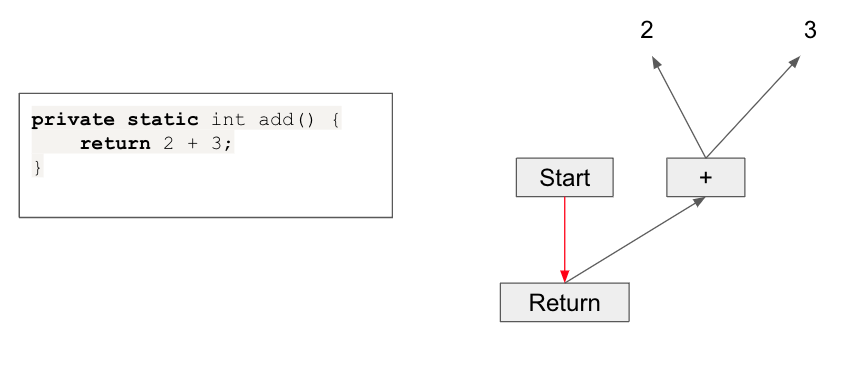
\includegraphics[width=1\textwidth]{Packages/graphir.png}
    \caption{Simple IR Graph}
    \label{figure:graphir}
\end{figure}

\autoref{figure:graphir} illustrates a simple IR graph, with control flow edges highlighted in red. The graph begins at the Start node, which connects to the Return node via a successor edge. Upon reaching the Return node, the graph traverses upward through data flow edges to compute the returned expression’s value. This traversal demonstrates how control and data flows interact to process and complete the function's execution.

\subsection{Prolog Programming Language}

In traditional imperative languages, a program consists of a sequence of instructions. This approach emphasizes a step-by-step procedure where each instruction modifies the state of the machine to solve a given problem. In contrast, logic programming languages, such as Prolog, operate on a fundamentally different paradigm. Instead of prescribing a sequence of operations, logic programming focuses on defining a knowledge base composed of facts and rules \cite{Bramer2013}. After that, users can query the knowledge base to search for objects and relations. 

In Prolog, facts represent objects and their relationships, while rules imply the relationship between objects given it satisfies all the conditions. Once the knowledge base is established, users can formulate queries to extract information or solve problems by leveraging the logical relationships defined in the base using the depth-first search algorithm \cite{Chowdhary2020}. There may be several ways to achieve a given goal. The system initially selects the first available option. If Prolog fails to resolve a specific subgoal, it will backtrack to explore these previously noted alternatives. This mechanism, referred to as backtracking \cite{Chowdhary2020}, enables Prolog to systematically search for different solutions by revisiting and trying alternative paths.

\begin{figure}[h]
    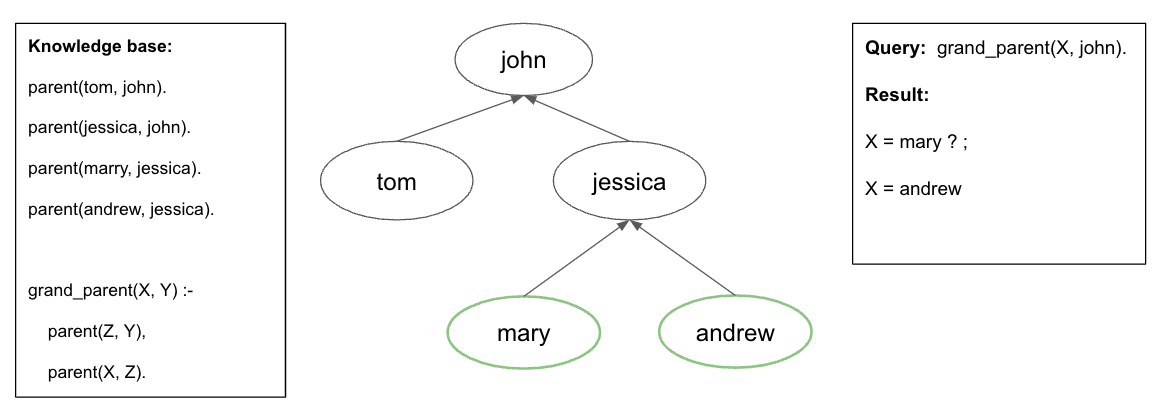
\includegraphics[width=0.95\textwidth]{Packages/Prolog.png}
    \caption{Example of Prolog specification}
    \label{figure:prolog}
\end{figure}

\autoref{figure:prolog}  illustrates a Prolog program. The first and final clauses are facts, specifying that nodeA is the parent of both nodeB and nodeC. In contrast, the intermediate clause represents a rule, which defines that nodeA is not the parent of nodeD. When a query is made to determine the nodes for which nodeA is a parent, Prolog executes a search from the first to the last clause, demonstrating its backtracking behavior.

\section{Literature Review}

\subsection{Advancements Through Domain-Specific Languages (DSLs)}
Declarative domain-specific languages (DSLs) have made a big impact on compiler optimization by offering targeted solutions for specific optimization tasks. For example, the Halide programming language improves image processing by separating the algorithm from its schedule, essentially the optimizations applied to the code \cite{Jonathan2018}. This separation allows for efficient and parallelized implementations with less manual effort. However, automating scheduling and keeping algorithms modular, especially as they grow in complexity, remains a challenge. Meanwhile, Spinellis created a peephole optimizer that uses a declarative DSL to specify optimizations \cite{Spinellis1999}. Spinellis transformed specifications into string regular expressions, which are then applied to the target code, allowing for adaptive and efficient refinements. Although this method has only been tested on smaller programs and specific types of optimizations so far, it shows great potential for quickly experimenting with new techniques and architectures. Elevate \cite{Hagedorn2020} is another functional language designed to let programmers define custom optimization strategies. It allows for creating composable optimizations rather than sticking to predefined APIs. Its success in case studies and practical applications highlights its ability to handle complex optimization tasks and deliver strong performance.

\subsection{Advancements Through Logic Programming Languages}
DataLog has established itself as a powerful tool in compiler implementation through its applications in complex program analysis and transformation. For instance, Lam et al. developed a framework using Datalog queries and a specialized language called PQL, which employs deductive databases and binary decision diagrams (BDDs) to tackle complex issues like pointer aliasing and heap object management in a context-sensitive manner \cite{Lam2005}. This approach has simplified the creation of sophisticated analyses and has been crucial in identifying security vulnerabilities in C and Java applications. Similarly, the Doop framework \cite{Bravenboer2009} utilizes Datalog to offer a declarative solution for points-to analysis in Java, providing impressive performance gains and scalability for precise context-sensitive analyses that were previously challenging to achieve. Furthermore, the Soufflé Datalog engine \cite{silverman2021wantanalyzeschemeprograms} introduces a new method for control-flow analysis in Scheme, making it possible to perform scalable and complex analyses of functional programming constructs, and extending the benefits of Datalog-based static analysis to Scheme-like languages. Finally, DIMPLE \cite{Benton2007}, a framework for Java bytecodes static analyses, is implemented in the Yap Prolog system. DIMPLE leverages logic programming capabilities to provide a declarative language for specifying analyses and representing Java bytecodes. The framework facilitates iterative experimentation and delivers efficient implementations that are on par with specialized tools.

\subsection{Transformation, Rewriting Techniques, and Verification}
Transformation and rewriting techniques are essential components of modern compiler optimization, enabling sophisticated processes like grammar specification, pattern matching, and program rewriting. Stratego \cite{Eelco2001} distinguishes between rewriting strategies and transformation rules, which allows for a highly flexible and controlled approach to applying optimization rules. The Stratego compiler translates these specifications into C code and leverages the ATerm library for effective term representation. It incorporates various optimizations, such as aggressive inlining and pattern merging, although it still encounters challenges related to compilation speed and support for separate compilation~\cite{Eelco2001}. On the other hand, Veriopt \cite{Webb2023} offers a comprehensive framework for formally verifying optimization rules used in the GraalVM compiler. This framework employs term rewriting rules on an abstract term representation and then maps these rules to term graph transformations. Veriopt has successfully validated 45 optimization rules for GraalVM’s intermediate representation, thus advancing the reliability and effectiveness of compiler optimizations.

\subsection{Identified Research Gaps}
Despite the established effectiveness of logic programming languages like Datalog in program analysis, there is limited research on integrating these techniques within modern compiler frameworks such as GraalVM. While significant advancements have been made in transformation and rewriting techniques using domain-specific languages (DSLs) and other paradigms, there is a notable absence of comparative studies on incorporating logic programming-based optimizations into GraalVM. This gap extends to a lack of empirical evidence assessing the impact of such techniques on optimization time and efficiency. Integrating Prolog-based rules with GraalVM’s graph-based IR is particularly challenging due to insufficient research on mapping Graal IR to Prolog and ensuring that Prolog-based optimizers work effectively within the Java environment. Addressing these challenges could enhance our understanding of how to apply logic programming in modern compilers and improve compiler optimization practices by providing valuable insights into the performance and effectiveness of these techniques.

\chapter[Literature Review]{Literature}

\section{Domain-Specific Languages (DSLs)}
Declarative domain-specific languages (DSLs) have made a big impact on compiler optimization by offering targeted solutions for specific optimization tasks. For example, Halide \cite{Jonathan2018} is a domain-specific language and compiler framework designed to optimize image processing and computational photography. Writing efficient code for image processing often requires complex optimizations to exploit parallelism and memory locality. In Halide, the algorithm specifies the computational logic for these tasks, detailing what needs to be done, such as resizing, sharpening, or blurring an image. The schedule defines the execution strategy, including how computations are ordered, parallelized, and managed in memory. This separation of concerns allows Halide to generate highly optimized code by focusing on both the functional description and the efficient execution of tasks. Elevate \cite{Hagedorn2020} is another functional language designed to let programmers define custom optimization strategies. It allows for creating composable optimizations rather than sticking to predefined APIs. Its success in case studies and practical applications highlights its ability to handle complex optimization tasks and deliver strong performance.

\begin{figure}[h]
    \centering
    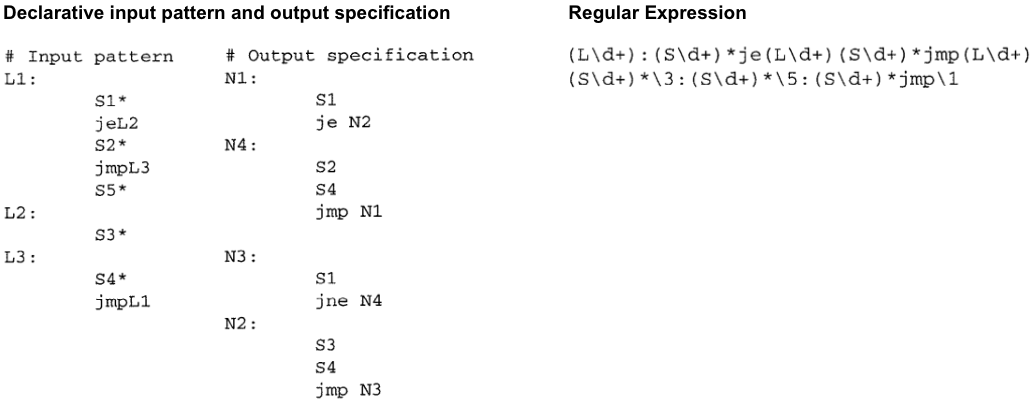
\includegraphics[width=1\textwidth]{Packages/regex.png}
    \caption{Example of Optimizer Patterns and Regular Expression \cite{Spinellis1999}}
    \label{figure:regex}
\end{figure}

Spinellis created a peephole optimizer that uses a declarative DSL to specify optimizations \cite{Spinellis1999}. Spinellis transformed specifications into string regular expressions, which are then applied to the target code, allowing for adaptive and efficient refinements. \autoref{figure:regex} illustrates an example of this framework. On the left of the figure is a declarative specification for the one-bit loop optimization \cite{Spinellis1999}. The input pattern is parsed and translated into the regular expression in the right part of the figure. The optimizer uses regular expressions to find matches in the program and transform and optimize the code iteratively.

\section{Logic Programming Languages}
DataLog has established itself as a powerful tool in compiler implementation through its applications in complex program analysis and transformation. For instance, the Soufflé Datalog engine \cite{silverman2021wantanalyzeschemeprograms} introduces a new method for control-flow analysis in Scheme, making it possible to perform scalable and complex analyses of functional programming constructs, and extending the benefits of Datalog-based static analysis to Scheme-like languages. Similarly, DIMPLE \cite{Benton2007}, a framework for Java bytecode static analyses, is implemented in the Yap Prolog system. DIMPLE leverages logic programming capabilities to provide a declarative language for specifying analyses and representing Java bytecodes. The framework facilitates iterative experimentation and delivers efficient implementations that are on par with specialized tools. 

Another example is the Doop framework \cite{Bravenboer2009} which utilizes Datalog to offer a declarative solution for points-to analysis in Java, providing impressive performance gains and scalability for precise context-sensitive analyses. \autoref{figure:doop} illustrates a Datadog rule that Doop uses to represent a call graph. The query finds and returns a call graph edge if all of the predicates inside \texttt{CallGraphEdge} are true. First, it queries the properties of the virtual method call \texttt{call} including its receive object \texttt{base}, \texttt{name}, and \texttt{descriptor}. After that, it queries the \texttt{heap} that this \texttt{base} object is pointing to and checks for the type of that \texttt{heap} object. Finally, it queries method lookups for the method that is being called from the \texttt{heaptype}.

\begin{figure}[h]
    \centering
    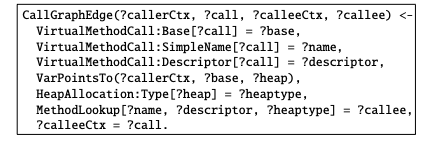
\includegraphics[width=0.6\textwidth]{Packages/Doop.png}
    \caption{DOOP's rule for virtual method invocations \cite{Bravenboer2009}}
    \label{figure:doop}
\end{figure}

Lam et al. developed a framework using Datalog queries and a specialized language called PQL, which employs deductive databases and binary decision diagrams (BDDs) to tackle complex issues like pointer aliasing and heap object management in a context-sensitive manner \cite{Lam2005}. PQL helps simplify the process by allowing programmers to write queries in a more intuitive way. Instead of needing to understand the underlying database details, programmers can write code patterns in Java that are automatically converted into Datalog. \autoref{figure:pql} provides an example of a query for simple SQL injection written in PQL and the equivalent Datadog rules. The SQL injection can be caught by checking if the parameter returned from calling \texttt{getParameter} on a \texttt{HttpServletRequest} is then passed directly as an argument to an \texttt{execution} call on the database \texttt{Connection}. Similarly, Datadog rules first check if there exists a method call to \texttt{getParameter} with a return value stored in a \texttt{v1} variable pointing to a heap object \texttt{h}. After that, it checks if there exists an invocation of \texttt{execute} with an argument \texttt{v2} also pointing to the object \texttt{h}.

\begin{figure}[h]
    \centering
    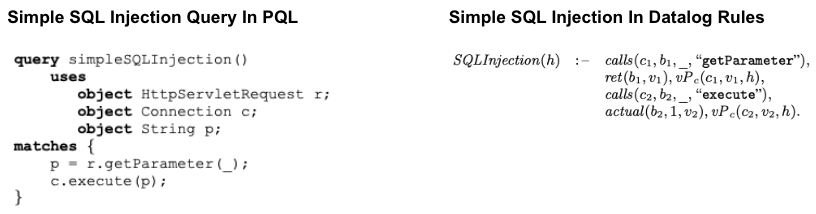
\includegraphics[width=1\textwidth]{Packages/PQL.png}
    \caption{Simple SQL Injection Example in PQL \cite{Lam2005}}
    \label{figure:pql}
\end{figure}

\newpage
\section{Transformation, Rewriting Techniques, and Verification}
Transformation and rewriting techniques are essential to modern compiler optimization, enabling sophisticated processes like grammar specification, pattern matching, and program rewriting. Stratego~\cite{Eelco2001} is a language designed for specifying program transformation systems using rewriting strategies, which allow for precise control over rule application. The compiler transforms these rules into C code and leverages the ATerm library for effective term representation. It has been used in several applications, including program transformation tools like XT, and domain-specific optimization frameworks like CodeBoost ~\cite{Eelco2001}. On the other hand, Veriopt \cite{Webb2023} offers a comprehensive framework for formal verification of Graal compiler optimizations. This framework employs  ``term rewriting rules on the abstract term representation" \cite{Webb2023} and then maps these rules to term graph transformations. In the Veriopt project, a term rewriting system, also known as an optimization phase, comprises a set of rules that can be applied repeatedly to optimize expressions. Each phase is associated with different types of root nodes in patterns, such as AddNode, AbsNode, and MulNode. 

\begin{figure}[h]
    \centering
    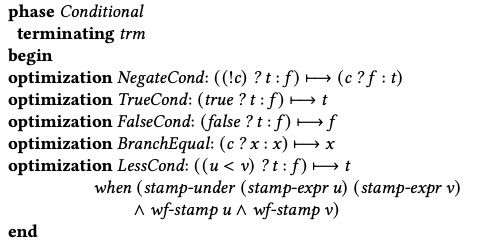
\includegraphics[width=0.6\textwidth]{Packages/veriopt.png}
    \caption{Conditional canonicalization rules \cite{Webb2023}}
    \label{figure:veriopt}
\end{figure}

\autoref{figure:veriopt} provides an example of such an optimization phase tailored for conditional expressions. NegateCond transforms negated conditions using logical equivalences, while TrueCond simplifies expressions where the condition is always true by directly applying the true outcome. Conversely, FalseCond addresses conditions that are always false by eliminating irrelevant branches. BranchEqual simplifies expressions with equality checks by optimizing or removing redundant comparisons.

\section{Identified Research Gaps}
Despite the established effectiveness of logic programming languages like Datalog in program analysis, there is limited research on integrating these techniques within modern compiler frameworks such as GraalVM. While significant advancements have been made in transformation and rewriting techniques using domain-specific languages (DSLs) and other paradigms, there is a notable absence of comparative studies on incorporating logic programming-based optimizations into GraalVM. This gap extends to a lack of empirical evidence assessing the impact of such techniques on optimization time and efficiency. Integrating Prolog-based rules with GraalVM’s graph-based IR is particularly challenging due to insufficient research on mapping Graal IR to Prolog and ensuring that Prolog-based optimizers work effectively within the Java environment. Addressing these challenges could enhance our understanding of how to apply logic programming in modern compilers and improve compiler optimization practices by providing valuable insights into the performance and effectiveness of these techniques.

\chapter[Project Plan]{Project Plan}

\section{Project Aims}
The aim of this project is to evaluate the potential of integrating a Prolog-based optimization framework within the GraalVM compiler. Logic programming languages have demonstrated significant advantages in the program analysis phase of compilers. This project seeks to explore their application in the optimization phase—a complex and critical component of the compiler. Enhancing the optimization phase could lead to substantial improvements in program speed and performance.

\textbf{Aims}
\begin{compactitem}
    \item \textbf{Develop Prolog-Based Optimization Rules:} Implement Prolog rules for various optimization techniques within the Ahead-of-Time (AOT) compiler.
    \item \textbf{Integrate Prolog-Based Optimization:} Assess the feasibility of incorporating a Prolog-based optimization framework within the GraalVM compiler.
    \item \textbf{Enhance Optimization Expressiveness:} Evaluate how Prolog can improve the expressiveness and effectiveness of compiler optimizations compared to existing GraalVM techniques.
    \item \textbf{Evaluate New Optimizations:} Investigate potential new optimizations enabled by Prolog specifications and compare their performance against existing GraalVM optimization methods.
\end{compactitem}

\setcounter{secnumdepth}{3}

\section{Methodology}

\subsection{Prolog-Based Optimization Framework}
The Prolog-based optimization framework is composed of three key components. 

\textbf{Prolog fact generator:} Generate Prolog facts that accurately represent the IR graph of the program. This component will parse the IR and convert it into a Prolog-compatible format, allowing Prolog rules to operate on the program's structure. The approach involves traversing the IR graph and generating Prolog facts based on the graph's nodes and edges.

\textbf{Prolog optimization rules:} Express optimization rules as Prolog facts and predicates. This involves translating optimization concepts into Prolog syntax, ensuring that the rules are both expressive and applicable to the GraalVM compiler's intermediate representation (IR).

\textbf{Prolog-based optimizer:} Recursively querying Prolog optimization rules, executing Prolog queries, and applying transformations to the IR. This system should iteratively refine the program based on the query results. The component will be developed in Java and could potentially leverage the GNU Prolog for Java library to facilitate the execution of Prolog queries within the Java environment. 

To ensure compatibility between Prolog facts and rules, the development of the first two components will occur in parallel.

\subsection{Integration Into GraalVM Compiler}
After developing the standalone components of the Prolog-based optimizer, the next step is to integrate it with the GraalVM compiler. GraalVM is a substantially large and very complex project. Therefore, this integration may encounter potential compatibility issues. It is necessary to treat the integration phase as a distinct part of the development process. This involves modifying the GraalVM compiler to interface effectively with the Prolog-based optimizer and ensuring that the compiler can pass IR data to the Prolog-based optimizer and receive optimized IR data back for further processing.

\subsection{Testing}
Since the optimization phases involve significant transformations to the original code, ensuring the soundness and correctness of the optimizer is crucial. To achieve this, a comprehensive test suite is developed to:
\begin{compactitem}
    \item \textbf{Verify Prolog Rules:} Test the Prolog rules to ensure they function correctly and identify all valid optimization opportunities without introducing errors.
    \item \textbf{Validate Fact Generation:} Confirm that the generated Prolog facts accurately represent the original Intermediate Representation (IR), ensuring consistency and correctness.
    \item \textbf{Assess Integration:} Evaluate the integration of the Prolog-based optimizer with the GraalVM compiler, ensuring that the optimized code accurately reflects the original code and that no errors are introduced during the optimization process.
\end{compactitem}

\subsection{Evaluation}
After validating the optimizer's correctness, performance must be evaluated and compared with existing methods to determine any improvements offered by Prolog-based optimizations. Additionally, it is important to assess whether the declarative syntax enhances documentation, comprehension, and maintenance of the optimizer.
\begin{compactitem}
    \item \textbf{Performance Metrics:} Measure various performance metrics including execution speed, resource utilization (e.g., memory and CPU), and optimization throughput. Compare these metrics with those of existing GraalVM optimization techniques to gauge improvements or regressions.
    \item \textbf{Strengths and Weaknesses:} Identify and document the strengths and weaknesses of the Prolog-based optimizer. This analysis will help in understanding how well Prolog-based optimizations perform relative to traditional methods and where improvements can be made.
    \item \textbf{Potential New Optimizations:} Explore and document potential new optimization techniques that can be enabled by Prolog specifications. This involves identifying unique optimization opportunities that Prolog's declarative nature may unlock, which are not feasible with traditional imperative methods. 
\end{compactitem}

\newpage

\section{Timeline}
The project timeline is divided into two parts: the first half (Semester 2, 2024) and the second half (Semester 1, 2025). The timeline is further divided into 4 phases: Project Proposal, Proof of Concept, Extension and Evaluation, and Report and Demonstration. The total duration of the project is 30 weeks, with a commitment of 10 working hours per week. The first half involves conducting research, writing the project proposal, and developing a proof of concept. The second half focuses on refining and expanding the project to encompass a comprehensive set of optimization rules, as well as preparing the final paper, report, and presentation. The timeline may be adjusted based on the results of the proof of concept phase to accommodate unforeseen challenges or to incorporate additional development needs.  The distribution of weeks per task is illustrated in the timeline graph below.

\begin{figure}[h]
    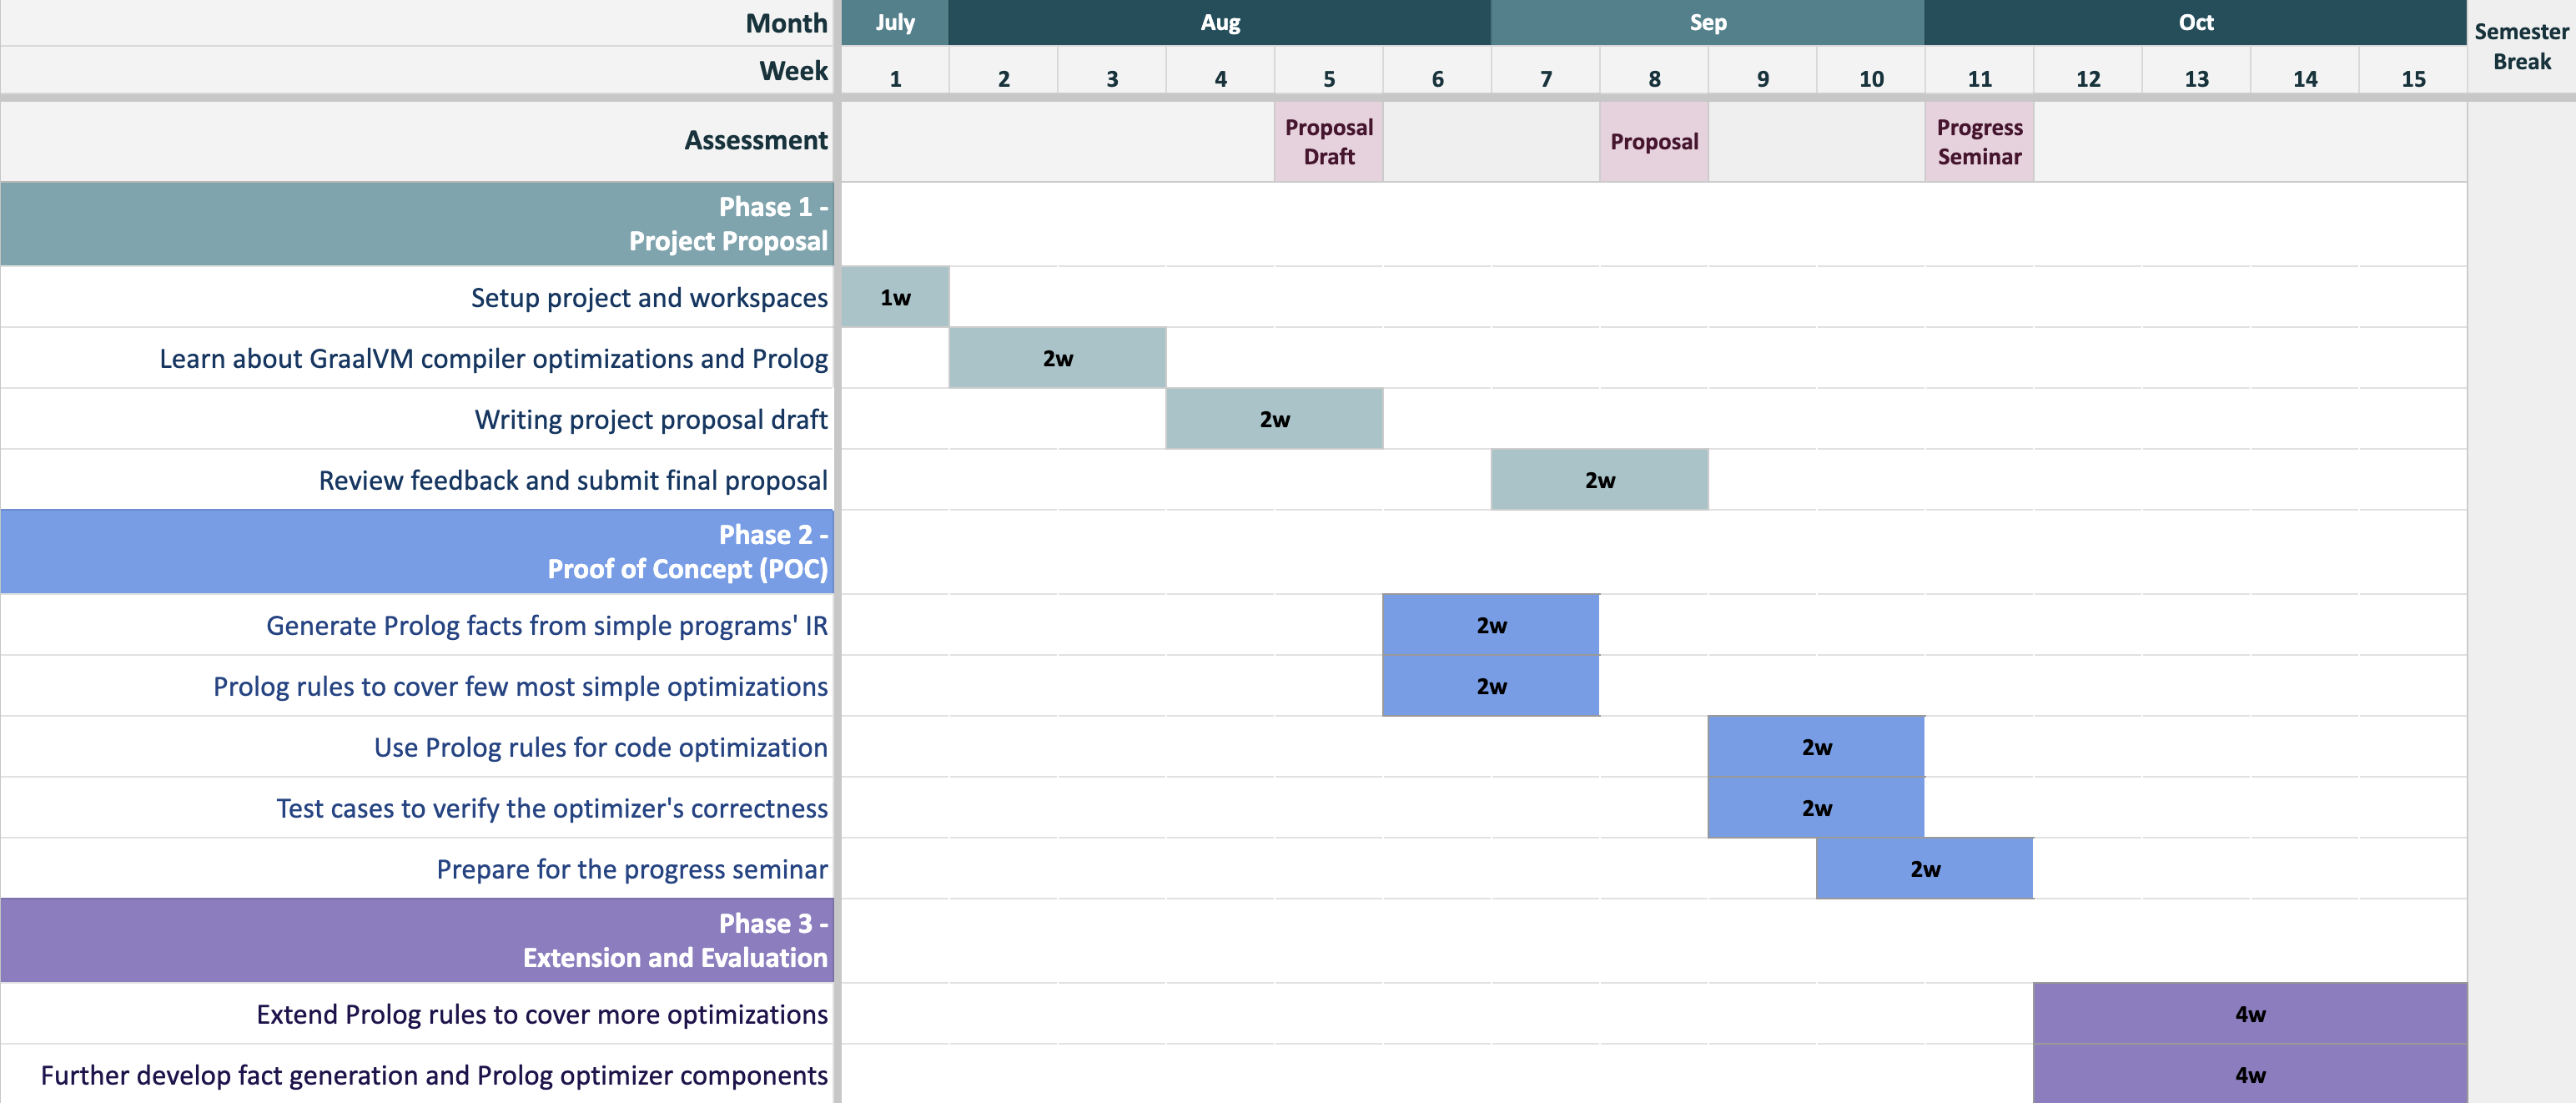
\includegraphics[width=1\textwidth]{Packages/PartA.png}
    \caption{Project Timeline (first half)}
\end{figure}
\begin{figure}[h]
    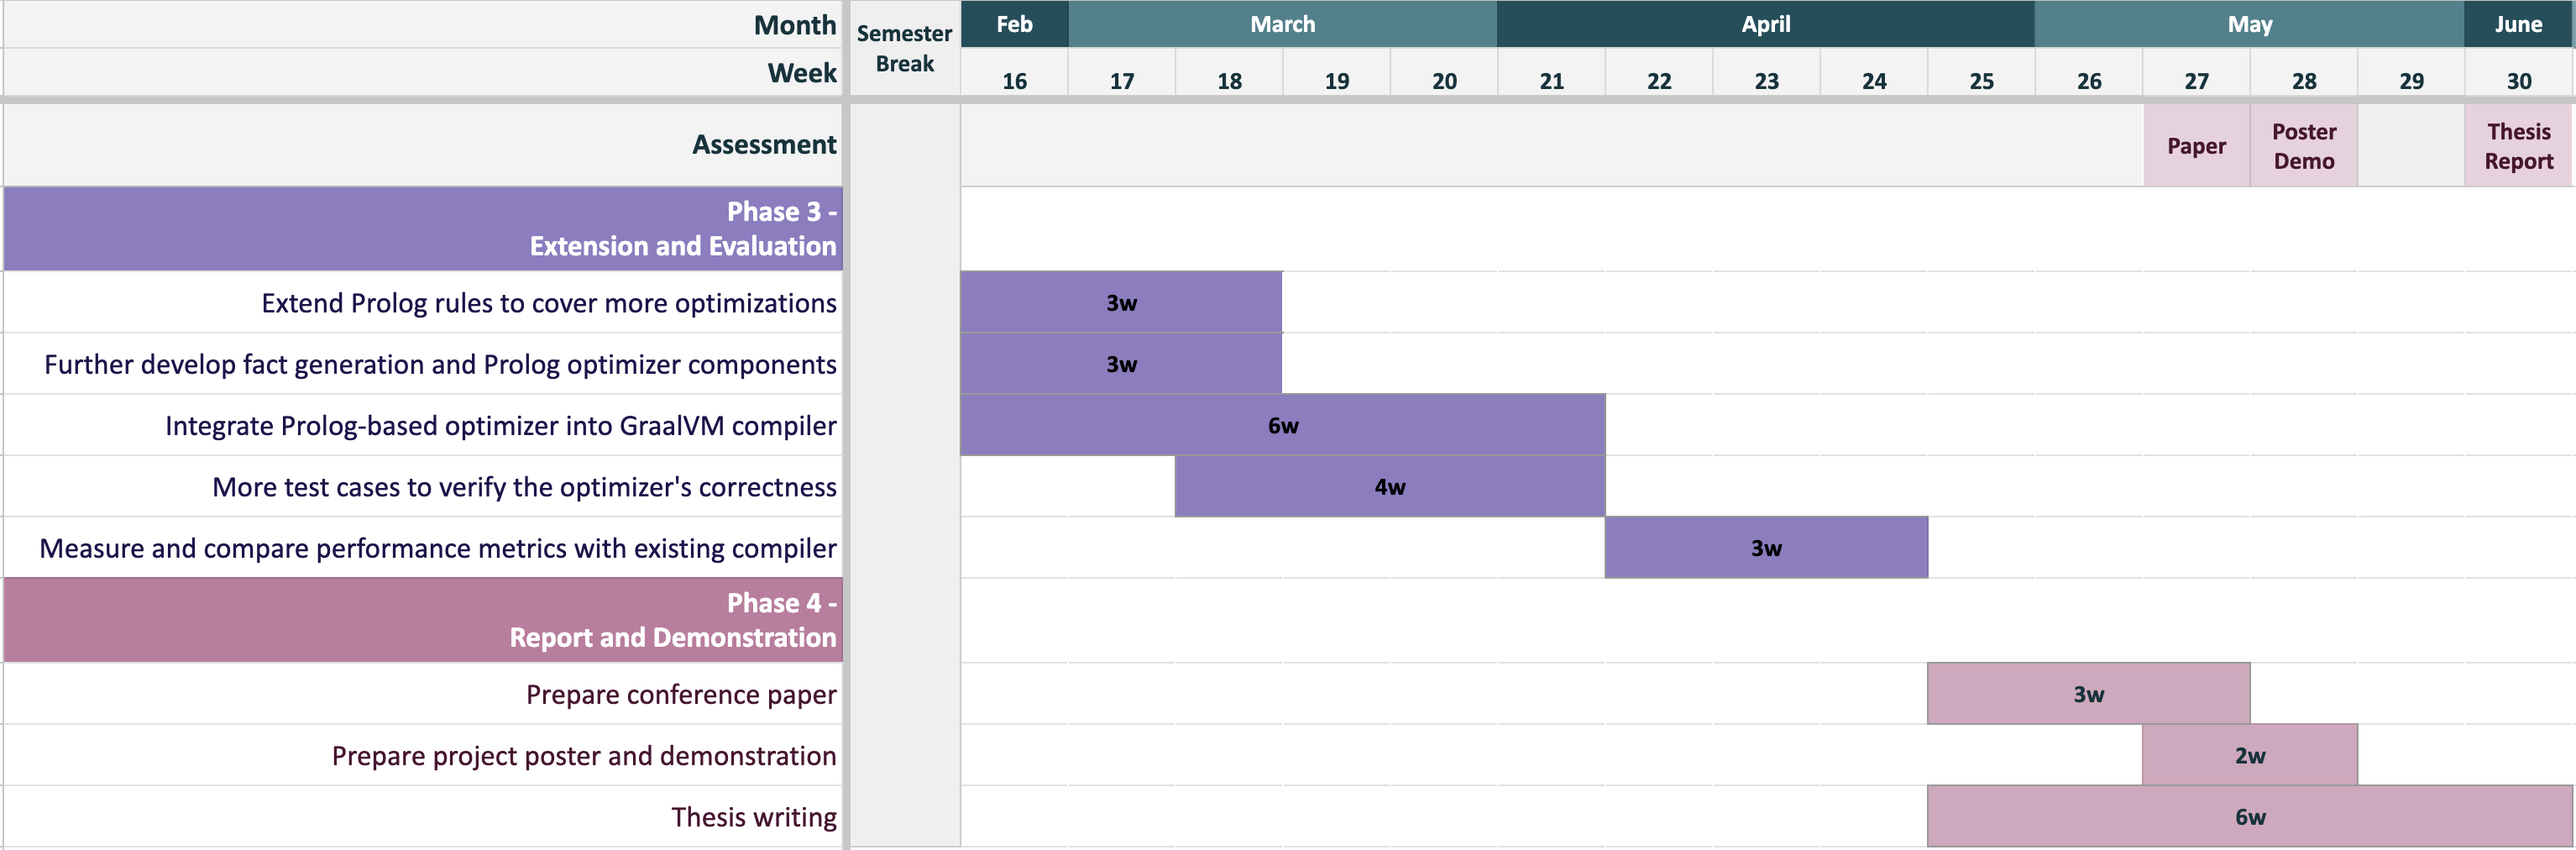
\includegraphics[width=1\textwidth]{Packages/PartB.png}
    \caption{Project Timeline (second half)}
\end{figure}

\newpage
Each project phase concludes with a milestone, except for the Extension and Evaluation phase, which includes two milestones due to a three-month semester break dividing this phase. The first three milestones occur during the first part of the project involve planning, validating the concept, and the initial development cycle. The final two milestones, scheduled for the second part, focus on advancing development and completing the final thesis.

\subsection{Milestone 1: Project Proposal}
\textbf{Date:} 19/09/2024 (Week 8) \\
\textbf{Deliveries:} Project proposal

To deliver the project proposal, several tasks need to be completed. The first week of the project involved meeting with the supervisors to gain a better understanding of the project and setting up the necessary tools and workspaces. The following two weeks focused on studying GraalVM compiler optimizations, intermediate representations (IR), and Prolog. The subsequent two weeks were dedicated to conducting additional research and a literature review in preparation for the draft proposal. Based on the feedback received, the final project proposal is expected to be delivered by the eighth week as an assessment item.

\subsection{Milestone 2: Proof of Concept (PoC) and Progress Seminar}

\textbf{Date:} 08/10/2024 (Week 11) \\
\textbf{Deliveries:} PoC and progress update presentation

In the second phase of the project, the focus will be on developing a proof of concept (PoC) for the Prolog-based optimizer. This PoC will employ a limited set of simple optimization techniques to assess the feasibility of the proposed approach. The PoC will also identify any additional development efforts required that may have been overlooked in the initial phase. Finally, this phase will conclude with a progress update seminar which is the second assessment item.

\subsection{Milestone 3: Initial Extension and Improvement Cycle}

\textbf{Date:} 01/11/2024 (Week 15) \\
\textbf{Deliveries:} More comprehensive set of optimization rules and a better Prolog-based optimizer

In the third phase, the focus will shift to extending and refining the proof of concept (PoC). Following the initial verification of optimization rules, efforts will be directed toward expanding the Prolog optimization rule sets to support more complex and advanced optimizations. Additionally, components such as the Prolog fact generator and the Prolog-based optimizer, will be revised and enhanced for increased robustness and efficiency, incorporating insights gained from the PoC results. The phase will conclude at the end of the semester, with a more comprehensive set of optimization rules and an improved optimizer from the previous phase.

\subsection{Milestone 4: Completion of Development and Testing}

\textbf{Date:} 25/04/2025 (Week 24) \\
\textbf{Deliveries:} Final version of the Prolog-based optimizer

The second half of the project will focus on continuing and enhancing the Prolog-based optimizer based on insights from the previous phase. A key objective will be to integrate the Prolog-based optimizer with the GraalVM compiler. This phase will also involve developing comprehensive test cases to ensure the optimizer’s correctness and robustness. Performance metrics will be assessed and compared with those of the existing GraalVM compiler to identify strengths and weaknesses. The phase will conclude with the finalization of the Prolog-based optimizer and a detailed review of its capabilities, performance, and potential for future enhancements.

\subsection{Milestone 5: Thesis Writing and Demonstration}
\textbf{Date:} 09/06/2025 (Week 30) \\
\textbf{Deliveries:} Final thesis report

With all development and testing completed in the previous phase, the final phase of the project will focus on preparing the conference paper, project poster, project presentation, and final thesis report, which are the remaining assessment items. The submission of the final thesis report will mark the project's completion.

\newpage

\section{Ethics \& Risk Assessment}
\subsection{Ethics Assessment}
This project exclusively engages with software and does not involve the collection or use of data from human or animal subjects. As a result, it does not require any substantial ethical considerations.
\subsection{Risk Assessment}
The table below outlines potential risks that could impact project success, along with corresponding mitigation strategies to minimize their likelihood and severity.
\renewcommand{\arraystretch}{1.3}
\begin{table}[h]
    \begin{tabularx}{1\textwidth} { 
        | >{\raggedright\arraybackslash}p{8em}
        | >{\raggedright\arraybackslash}p{4.5em} 
        | >{\raggedright\arraybackslash}p{4.5em} 
        | >{\raggedright\arraybackslash}p{3.5em} 
        | >{\raggedright\arraybackslash}X 
        | 
        }   
        \hline
        \textbf{Risk} & 
        \textbf{Likelihood} & 
        \textbf{Severity} & 
        \textbf{Risk Level} &
        \textbf{Mitigation Strategy}
        \\ 
        \hline
        Unable to meet key requirements and lagging behind scheduled milestones.
        & Possible & Significant & High & 
        Conduct regular meetings with supervisors and team members to assess project progress, identify and resolve any obstacles or difficulties, and ensure efficient time management.
        \\ 
        \hline
        Loss development progress due to computer problem.
        & Unlikely & Significant & Medium & 
        Backup all work progress to multiple places, e.g. code to GitHub and reports to drive.
        \\ 
        \hline
        Insufficient expertise in logical programming languages and the GraalVM compiler.
        & Likely & Minor & Medium &
        Dedicate time to acquiring domain knowledge and studying Prolog, GraalVM optimizations, and intermediate representation (IR) constructs. Consult supervisors regularly for guidance and support.
        \\ 
        \hline
        The Prolog-based optimizer may be less accurate and add performance overhead.
        & Possible & Moderate & Medium &
        Develop various test cases, conduct benchmarking to assess optimizer performance, and analyze the accuracy of the results.
        \\ 
        \hline
        Health issues while working with the project.
        & Possible & Moderate & Medium &
        Ensure that the project is systematically organized and well paced to prevent overwork and mitigate stress.
        \\ 
        \hline
        Safety issues in the workplace.
        & Unlikely & Minor & Low &
        Safety concerns are limited, given that the work is conducted in a controlled, in-house environment and involves only computer systems.
        \\ 
        \hline
    \end{tabularx}
\caption{Risk Assessment.}
\end{table}



\bibliographystyle{IEEEtran}

\bibliography{./References/Bibliography}

\end{document}
